%! TEX root = main.tex
\documentclass[main.tex]{subfiles}
\begin{document}
\subsection{Laser-Metal-Deposition}
Laser-Metal-Deposition (LMD), auch bekannt als Directed-Energy-Deposition, ist ein weiteres Metall-3D-Druck-Verfahren. LMD ist ein Überbegriff für Schweißraupen-basiertes Additive Manufacturing, da viele weitere Verfahren existieren wie Electron-Beam-Melting.
\begin{figure}[h!]
	\begin{center}

		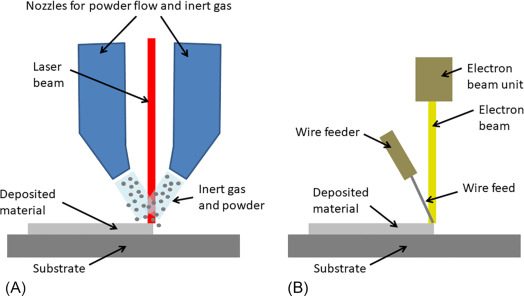
\includegraphics{lmd_1}
\ccaption{Aufbau zweier LMD-Konzepte}{\url{https://ars.els-cdn.com/content/image/3-s2.0-B9780081026632000022-f02-04-9780081026632.jpg}}
\label{img:lmd_1}	
	\end{center}
\end{figure}
Abb. \ref{img:lmd_1} zeigt die beiden wichtigisten Verfahren dieser Übergruppe: (a) Laser-DED \& (b) Electron-Beam-DED.
Bei (a) wird das Druckmaterial durch die Düse dem Laser zugeführt, welcher es dann auf das bereits darunterliegende Material aufträgt. 
Dagegen wird bei (b) mithilfe eines Elektronen-Strahls ein Draht aufgeschmolzen und in dieser Form aufgetragen. \parencite{ALL3D_1}
\subsection{Mehrachsen- \& Hybrid-Maschinen}
Da besagte Schweißraupen nicht genau den Modell folgend geformt werden können und deswegen oft mit einer rauen Oberfläche gedruckt werden werden in der industriellen Umgebung sogenannte Mehrachsen- sowie auch Hybrid-Maschinen beliebter. Diese verbinden den herkömmlichen LMD-Drucker mit den Fräß- und Nachbearbeitungsfähigkeiten einer CNC-Fräßmaschine (Computerized-Numerical-Control) um die Nachbearbeitung sofort in den Prozess einzufügen.

Die zusätzlichen Achsen der Maschine ermöglichen es, nicht nur Schichtweise aufzutragen, sondern auch an schiefen Elementen, nachdem diese bereits gedruckt wurden oder an bereits existierenden Teilen für sogenanntes Additive Remanufacturing, also der Reperatur konventionell hergestellter Teile. \parencite{ALL3D_2}
\begin{figure}[h!]
	\begin{center}
	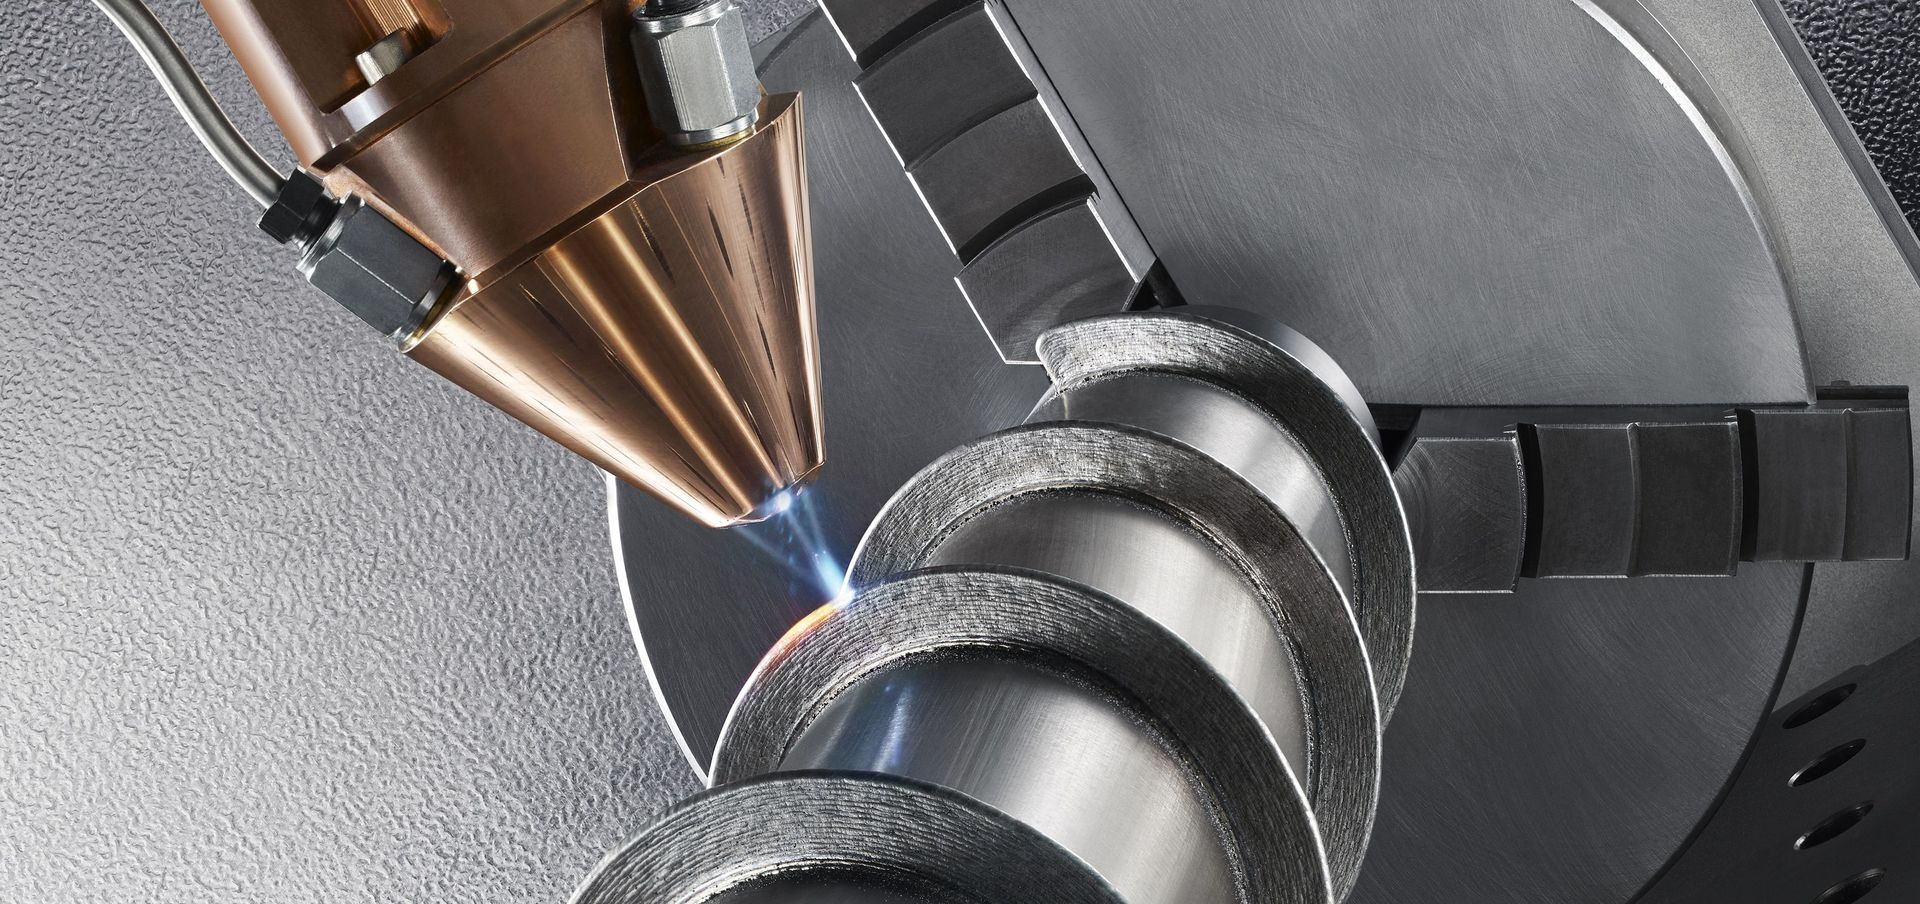
\includegraphics[width=0.8\textwidth]{lmd_part_1}	
		\ccaption{LMD Teil in Produktion auf Drehachse}{\url{https://www.trumpf.com/filestorage/TRUMPF_Master/_processed_/b/c/csm_Lasers-applications-laser-metal-deposition-process_37a1adacb9.jpg}}
		\label{img:lmd_part_1}
	\end{center}
	
\end{figure}

LMD kann auch verwendet werden um Teile für alte Maschinen zu reparieren, für welche die Ersatzteile nicht mehr in Produktion sind.
Abb. \ref{img:lmd_part_1} zeigt ebendies bei einer Stange, auf welche auf einer Drehachse ein Gewinde neu aufgetragen wird. 

\end{document}

